\documentclass{beamer}

\usepackage{color}
\usepackage{listings}
\lstset{
  frame=single,language=bash,
  morekeywords={od, in, foreach, let, end, and, or, proc, while},
   basicstyle=\footnotesize,
  escapechar=\@,
  basicstyle=\footnotesize, frame=tb,
  numbers=left,
  stepnumber=2,
  numbersep=5pt, 
  numberstyle=\tiny\color{mygray},
  xleftmargin=.2\textwidth, xrightmargin=.2\textwidth
}
\definecolor{bluekeywords}{rgb}{0.13,0.13,1}
\definecolor{greencomments}{rgb}{0,0.5,0}
\definecolor{redstrings}{rgb}{0.9,0,0}
\definecolor{mygray}{rgb}{0.2,0.2,0.2}

\usepackage{tikz}
\usetikzlibrary{positioning}
\usetikzlibrary{arrows,automata}

% There are many different themes available for Beamer. A comprehensive
% list with examples is given here:
% http://deic.uab.es/~iblanes/beamer_gallery/index_by_theme.html
% You can uncomment the themes below if you would like to use a different
% one:
%\usetheme{AnnArbor}
%\usetheme{Antibes}
%\usetheme{Bergen}
%\usetheme{Berkeley}
%\usetheme{Berlin}
%\usetheme{Boadilla}
%\usetheme{boxes}
%\usetheme{CambridgeUS}
%\usetheme{Copenhagen}
%\usetheme{Darmstadt}
\usetheme{default}
%\usetheme{Frankfurt}
%\usetheme{Goettingen}
%\usetheme{Hannover}
%\usetheme{Ilmenau}
%\usetheme{JuanLesPins}
%\usetheme{Luebeck}
%\usetheme{Madrid}
%\usetheme{Malmoe}
%\usetheme{Marburg}
%\usetheme{Montpellier}
%\usetheme{PaloAlto}
%\usetheme{Pittsburgh}
%\usetheme{Rochester}
%\usetheme{Singapore}
%\usetheme{Szeged}
%\usetheme{Warsaw}
\usecolortheme{lily}

\title{02257 Applied functional programming}

% A subtitle is optional and this may be deleted
\subtitle{Project debriefing}

\author{Kim Rostgaard Christensen}

\institute[Techical University of Denmark] % (optional, but mostly needed)
{
  
  DTU Compute\\
  Techical University of Denmark}

\date{Jan. 22. 2015}

\subject{Project work overwiew}
% This is only inserted into the PDF information catalog. Can be left
% out. 

% If you have a file called "university-logo-filename.xxx", where xxx
% is a graphic format that can be processed by latex or pdflatex,
% resp., then you can add a logo as follows:
\pgfdeclareimage[height=0.8cm]{university-logo}{dtu-compute-logo.jpg}
\logo{\pgfuseimage{university-logo}}

\begin{document}

\begin{frame}
  \titlepage
\end{frame}

\begin{frame}[plain,c]
\begin{center}
\Huge Project 1\\
\vspace{5mm}
\Large WHILE interpreter
\end{center}
\end{frame}

\section{Project 1 - WHILE interpreter}
\subsection{Project state}

\begin{frame}{WHILE interpreter}{State of the project}
  \begin{itemize}
  \item {
    Handed out cases passing
  }
  \item {
    Recursive and non-recursive function declarations
  }
  \item {
    Array operations
  }
  \pause
  \item {
    And..
  }
  \end{itemize}
\end{frame}

\subsection{Extensions}
\begin{frame}{WHILE interpreter}{Extensions}
  \begin{itemize}
  \item {
    For loops
  }
  \item {
    Syntactic sugarcoating - foreach loops
  }
  \item {
    Infix logic operators \alert{\texttt{and}} and \alert{\texttt{or}}
  }
  \end{itemize}
\end{frame}

\begin{frame}[fragile]{WHILE interpreter}{Extension - for loops}

\begin{figure}
\begin{lstlisting}
for (@$stmt_{init}$@; @$expr_{cond}$@; @$stmt_{incr}$@) do
  @$stmt_{body}$@
od
\end{lstlisting}
\caption{For loop}
\end{figure}

\begin{figure}
\begin{lstlisting}
let
  @$stmt_{init}$@
in
while @$expr_{cond}$@ do 
  @$stmt_{body}$@
  @$stmt_{incr}$@
od
end
\end{lstlisting}
\caption{Equivalent while loop (Block)}
\end{figure}
\end{frame}

%\begin{frame}[fragile]{WHILE interpreter}{Extension - sugarcoating}
%\begin{figure}
%  \begin{lstlisting}
%foreach @$var_{element}$@ in @$var_{array}$@ do
%  @$stmt_{body}$@
%od
%\end{lstlisting}
%\caption{Foreach loop}
%\end{figure}

%\begin{figure}
%\begin{lstlisting}
%let
%  _rewrite : 
%in
%@$stmt_{init}$@
%while @$expr_{cond}$@ do 
%  @$stmt_{body}$@
%  @$stmt_{incr}$@
%od
%end
%\end{lstlisting}
%\caption{Equivalent while loop (Block)}
%\end{figure}
%\end{frame}

\begin{frame}[fragile]{WHILE interpreter}{Extension - infix logic operators}
\begin{figure}
\begin{lstlisting}
let
  isNumber_a : isInt(a) or isFloat(a);
  ...
in
  if isNumber_a and isDefined (a) then
    ...
  fi
end
\end{lstlisting}
\caption{Infix logic operator example}
\end{figure}
\end{frame}

\begin{frame}{WHILE interpreter}{Reflections}
  \begin{itemize}
  \item {
    Very interesting applied project, good match for functional language
  }
  \item {
    Possible extensions
  }
  \begin{itemize}
    \item Stronger typing and/or type inference
    \item Static analysis functions (from Program analysis course)
    \end{itemize}
  \end{itemize}
\end{frame}

\section{Project 2 - Tree drawing}
\begin{frame}[plain,c]
\begin{center}
\Huge Project 2\\
\vspace{5mm}
\Large Tree drawing
\end{center}
\end{frame}
\subsection{Project state}
\begin{frame}{Tree drawing}{State of the project}
  \begin{itemize}
  \item {
    Draws from fixed point on canvas (no auto-aligning of tree)
  }
  \item {
    Centralized labels
  }
  \item {
    Translates AST's from Project 1 into either
      \begin{itemize}
        \item an elaborate format mapped almost directly to AST with a deep tree structure or,
        \item a simplified format that merges information from several nodes.
     \end{itemize}       
  }
  \end{itemize}
\end{frame}


\subsection{Example}
\begin{frame}{Tree drawing}{Example tree}
\includegraphics[width=1.00\textwidth]{treeprint_example}
\end{frame}

\subsection{Extensions}
\begin{frame}{Tree drawing}{Extensions}
  \begin{itemize}
  \item {
    No extensions :-(
  }
  \pause
  \item {
    It took a few iterations to get the algorithm translated
  }
  \end{itemize}
\end{frame}

\begin{frame}{Tree drawing}{Reflections}
  \begin{itemize}
%  \item {
%    Very interesting applied project, good match for functional language
%  }
  \item {
    Possible extensions
  }
  \begin{itemize}
    \item PostScript macro possibilities
    \item Bounding boxes for label containers
    \end{itemize}
  \end{itemize}
\end{frame}
\section{Project 3 - Graphical UI}
\begin{frame}[plain,c]
\begin{center}
\Huge Project 3\\
\vspace{5mm}
\Large Graphical game UI
\end{center}
\end{frame}


\subsection{Project state}
\begin{frame}{Graphical NIM game}{State of the game}
  \begin{itemize}
  \item {
    Playable with AI opponent
  }
  \item {
    Modularized by files and -- to some extent -- design pattern
  }
  \item {
    Not all edge cases are covered, and some UI components still carry state
  }
  \end{itemize}
\end{frame}

\subsection{Project state}
\begin{frame}{Graphical NIM game}{States of the game}
\begin{center}
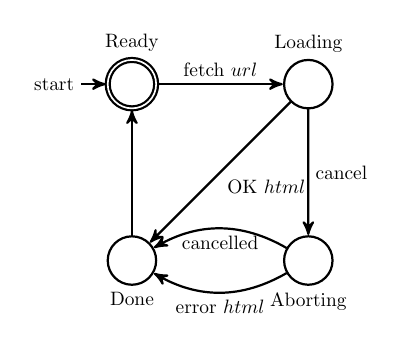
\begin{tikzpicture}[>=stealth',shorten >=0.2pt,auto,node distance=3.2cm,thick,scale=0.7, every node/.style={scale=0.7}]
  \node[initial,state,accepting,label=above:Ready] (Ready)                       {};
  \node[state,label=above:Loading]                 (Loading)  [right of=Ready]   {};
  \node[state,label=below:Aborting]                (Aborting) [below of=Loading] {};
  \node[state,label=below:Done]                    (Done)     [below of=Ready]   {};

  \path[->]
        (Ready) edge              node {fetch $url$}  (Loading)
      (Loading) edge              node {cancel}       (Aborting)
     (Aborting) edge [bend left]  node {error $html$} (Done)
     (Aborting) edge [bend right] node {cancelled}    (Done)
      (Loading) edge              node {OK $html$}    (Done);
  \path[->,label]
         (Done) edge              node {}             (Ready); 
\end{tikzpicture} \hspace{2mm} 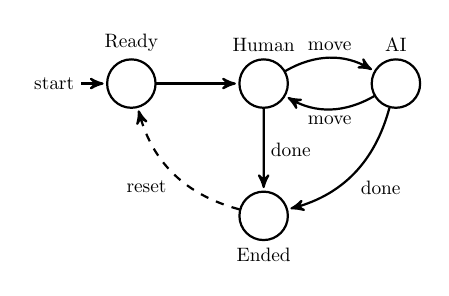
\begin{tikzpicture}[>=stealth',shorten >=1pt,auto,node distance=2.4cm,thick,scale=0.7, every node/.style={scale=0.7}]
  \node[initial,state,label=above:Ready] (Ready)                   {};
  \node[state,label=above:Human]         (Human)  [right of=Ready] {};
  \node[state,label=above:AI]            (AI)     [right of=Human] {};
  \node[state,label=below:Ended]         (Ended)  [below of=Human] {};


  \path[->]
     (Ready)  edge              node {} (Human)
      (Human) edge [bend left]  node {move} (AI)
        (AI)  edge [bend left] node {done} (Ended)
        (AI)  edge [bend left]  node {move} (Human)
      (Human) edge  node {done} (Ended);
  \path[->, dashed]
      (Ended) edge [bend left] node {reset} (Ready); 
\end{tikzpicture}
\end{center}
\end{frame}

\subsection{Project state}
\begin{frame}{Graphical NIM game}{Extensions}
  \begin{itemize}
  \item {
    Graphical representation of match heaps
  }
  \item {
    Strong separation of GUI components by responsibilities
  }
  \item {
    Multiple rounds of game, and launching of different games
  }
  \item {
    Multiple difficulties (predefined probabilities of making a random move)
  }
  \end{itemize}
\end{frame}

\begin{frame}{Graphical NIM game}{Graphical interfaces}
\begin{center}
\includegraphics[width=0.49\textwidth]{launcher_ui} \includegraphics[width=0.49\textwidth]{game_ui}
\end{center}
\end{frame}

\begin{frame}{Graphical NIM game}{Reflections}
  \begin{itemize}
  \item {
    Functional Reactive Programming is a suitable method for constructing user interfaces without distributed state everywhere
  }
  \item {
    Possible extensions
  }
    \begin{itemize}
      \item Extend the \texttt{AsyncEventQueue} to support multicast
      \item Represent state machines as graphs combined with a (multicast) \texttt{AsyncEventQueue} to enable a cleaner MVC pattern
    \end{itemize}
  \end{itemize}
\end{frame}

\begin{frame}[plain,c]
\begin{center}
\Huge EOT\\
\end{center}
\end{frame}
\end{document}